\section{Foundations and Taxonomy of Agentic Recommender Systems}
\label{sec:foundations-taxonomy}

{This section unifies two goals: (i) formalize agentic recommendation as an \emph{interactive decision process} and
define the entities we study (agents and agentic recommender systems) in \S \ref{subsec:recommender_as_interactive_decision}, and (ii) introduce a taxonomy that can organize
a rapidly growing literature beyond conventional RS task/method categorizations in \S \ref{subsec:two-axis-taxonomy-rewrite}.}

\subsection{Recommender systems as interactive decision processes}
\label{subsec:recommender_as_interactive_decision} 


Classical recommender systems are often presented as static mapping functions that produce a ranked list given a user and context. Agentic recommender systems (ARS), in contrast, are more naturally modeled as \textit{interactive decision processes} in which the system repeatedly observes a user’s requests and feedback, consults internal state and external resources, and decides what to do next. This shift is not merely a different UI; it changes what should be considered “the recommender”: the recommender becomes an \textit{entity that chooses actions} (\eg ask a question, retrieve candidates, apply constraints, call tools, verify a plan, generate an explanation), rather than a single-shot ranker.

To make this explicit, we view recommendation as proceeding in discrete turns \(t = 1, 2, \dots\). Let \(u_t\) denote the user input at turn \(t\) (which could be a query, constraints, or feedback). Let \(h_t = (u_1, y_1, \dots, u_t)\) denote the interaction history up to the current turn, where \(y_t\) is the system output (\eg recommendation response, clarification question, or tool-triggered result). In agentic settings, the system also maintains an internal state \(s_t\), which includes {user/item profiles}, {memory}, and other latent variables required for long-horizon consistency. 
The system chooses an action \(a_t\) from an action space \(\mathcal{A}\). Importantly, \(\mathcal{A}\) is not restricted to “recommend item \(i\).” 
It typically includes: 
\textit{dialogue actions} (ask, confirm, explain, negotiate trade-offs), \textit{tool actions} (retrieve, rank, filter, query a KB, browse the web), \textit{environment actions} (\eg add to cart, reserve, schedule) when in scope.




In the following, we define the LLM agent and agentic recommender, respectively. 
\vspace{2pt}
\begin{definition}[LLM Agent for Recommendation]
An LLM agent is an entity that repeatedly (i) \textbf{observes} an input comprising user signals and environment/tool outputs, (ii) \textbf{reasons} to interpret goals and constraints, (iii) optionally \textbf{plans} a sequence of actions, (iv) \textbf{acts} by producing user-facing outputs and/or invoking tools, and (v) \textbf{updates} its state (profile/memory) based on new evidence.
\end{definition} 
We represent an LLM agent as $A = (\mathcal{L}_\theta, \pi, \mathcal{P}, \mathcal{M}, \mathcal{T})$, where $\mathcal{L}_\theta$ is the LLM (or foundation model) used as the main reasoning engine.
\(\pi\) is the {controller/policy} that determines how the LLM is prompted, how tool calls are formatted/parsed, and how multi-step execution proceeds (\eg ReAct). 
Different workflows are detailed in \S~\ref{subsubsec:agent_rec_workflow}. 
\(\mathcal{P}\) is the {profile module} (persistent traits and summaries of the user and/or items). 
\(\mathcal{M}\) is the {memory module} (a store of episodic and/or semantic information used across turns and sessions). 
\(\mathcal{T}\) is the {tool set} (retrieval, ranking services, search engines, KB queries, etc.), along with a tool interface that maps agent outputs to executable calls.



\begin{definition}[Agentic Recommender System, ARS]
An agentic recommender system is an interactive recommendation system that contains one or more LLM agents that can plan and act using tools and memory to produce personalized outcomes. 
We formalize: $ARS = (\mathcal{U}, \mathcal{I}, \mathcal{E}, \mathcal{R}, \mathcal{A})$, 
where \(\mathcal{U}\) is the set of users, \(\mathcal{I}\) is the item universe, \(\mathcal{E}\) is the external environment (web, APIs, KBs, simulators), \(\mathcal{R}\) denotes classical RS components (optional; present in agent-assisted ARS), and \(\mathcal{A}=\{A_1, \dots, A_n\}\) is the set of agents.
\end{definition}


This definition is intentionally broad enough to cover three recurring paradigms in the literature: \textbf{agent-assisted recommendation}, \textbf{agent-as-recommender}, and \textbf{agent-as-user-simulator}. In this survey, we describe this role-based partition and ties it to LoA levels, which is detailed in \S~\ref{subsec:two-axis-taxonomy-rewrite}. 




\subsection{Why agentic systems require a new taxonomy}
\label{subsec:new-taxonomy-rationale}
{
Conventional taxonomies in recommender systems have focused on algorithmic families (matrix factorization versus neural networks), task categories (retrieval, ranking, reranking) or data modalities.  While such classifications were adequate for static pipelines, they struggle to describe the emergent landscape of \emph{agentic recommenders}.  In these systems the recommender is no longer a single‑shot scorer but an entity that can observe, reason, plan and act over multiple turns.  Agents can occupy different roles within the recommendation loop—sometimes augmenting a classical model with retrieval or constraint reasoning, sometimes replacing it entirely, and sometimes simulating users or environments to generate feedback for training and evaluation.  Two systems trained on the same dataset may therefore differ radically in how they treat an agent: one may rely on an agent merely to translate natural language into search queries, while another may delegate all decision‑making to the agent.  These differences affect the action space, interaction protocol, and evaluation methodology; they cannot be captured by algorithmic labels alone.  A new taxonomy must therefore capture both \emph{where} the agent is positioned within the recommendation pipeline and \emph{what} the agent is allowed to do, providing a framework that unifies agentic augmentation, agentic replacement, and agentic simulations.
}

\subsection{A two‑axis taxonomy: roles and autonomy levels}
\label{subsec:two-axis-taxonomy-rewrite}
{
To organise the burgeoning literature, we propose a two‑dimensional taxonomy that cross‑classifies agentic recommenders by \textbf{macro role}—the agent’s placement in the recommendation loop—and by \textbf{autonomy level}—the breadth of actions the agent can perform and the capabilities the agent can achieve. This structure clarifies relationships among systems that otherwise share similar datasets or metrics.
}


\begin{figure}[t]
% \vspace{-0.2cm}
\setlength{\abovecaptionskip}{0.02cm}
\setlength{\belowcaptionskip}{-0cm}
\centering
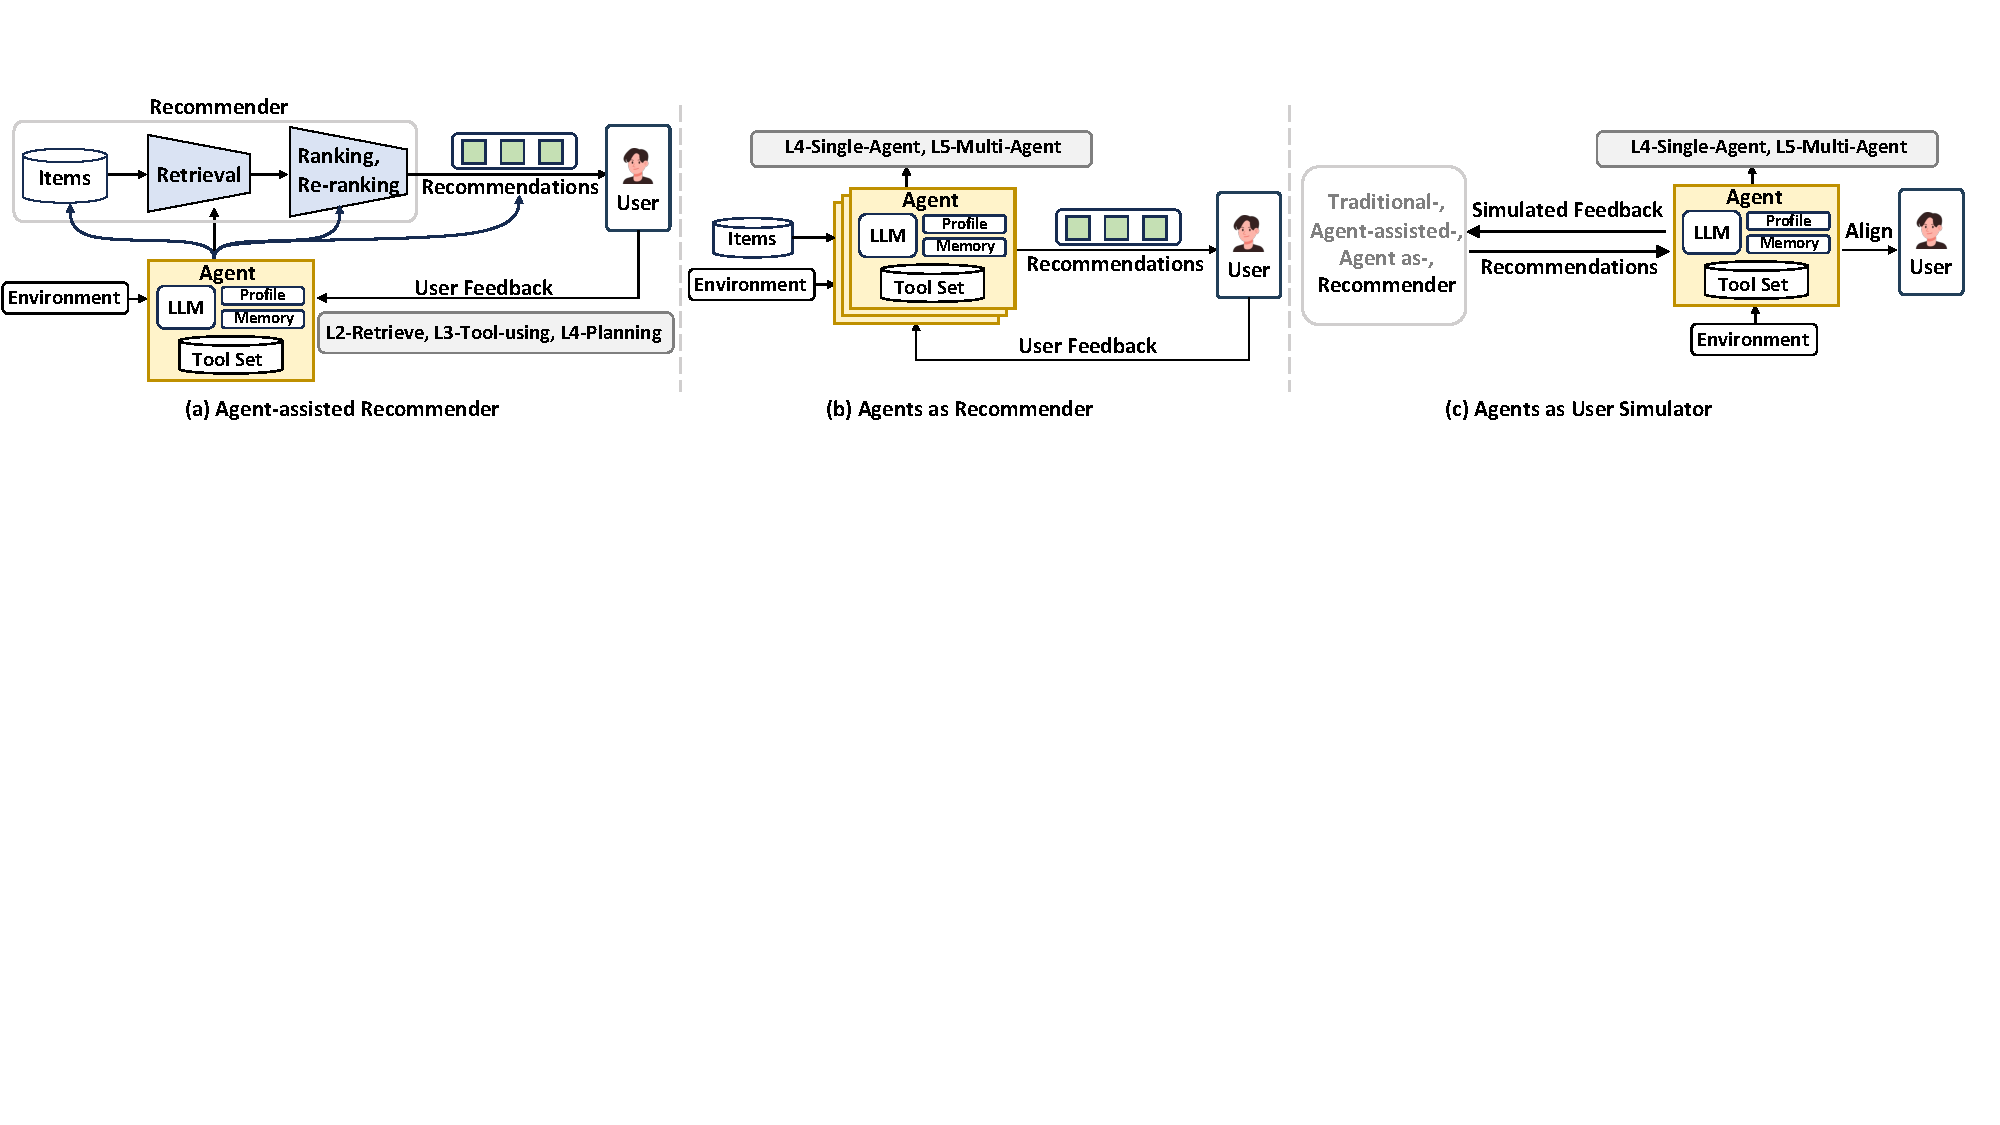
\includegraphics[width=0.99\linewidth]{figures/paradigm_comparison.pdf}
\caption{Illustration of three paradigms of agentic recommender systems. {While all of these variations make use of tools, memory, and user profiles, the main difference between (a) and (b) lies in whether they involve a classical retrieval component—\eg dense retrieval or collaborative-style retrieval as in (a)—or whether this process is handled by a single agent/LLM without the help of auxiliary retrieval modules, as in (b). In (c), agents simulate user behavior and provide simulated feedback to analyze or improve the recommender system. Thus, for example, in this view, we observe an agentic RAG workflow, where the agent is assisted by external tools, an LLM, and memory components to support retrieval and generation within the recommender pipeline.}}
\label{fig:paradigm_comparison}
\end{figure}

\paragraph{\textbf{Macro roles.}} We distinguish three high‑level roles as illustrated in Figure~\ref{fig:paradigm_comparison}:
\begin{enumerate}
  \item \textbf{Agentic augmentation}.  The agent works alongside a classical recommender, improving specific stages such as preference elicitation, evidence retrieval, or result filtering.  The classical model still produces the final ranking.  Systems like \emph{RecMind} and \emph{iAgent} fall here, where the agent interprets natural‑language queries and invokes retrieval or ranking tools but does not itself decide the top items.
  \item \textbf{Agentic replacement}.  One or more agents assume full responsibility for recommendation.  They maintain user state, orchestrate tool calls, retrieve and rank items, and generate explanations.  Classical models, if present, appear as tools rather than the primary controller.  Examples include \emph{InteRecAgent}, \emph{MADREC} and \emph{DRDT}, where an LLM agent decides both what to recommend and how to justify it.
  \item \textbf{Agentic simulation}.  Agents model the behaviour of users or environments, generating clicks, ratings, critiques or dialogue acts for training, evaluation and robustness analysis.  Multi‑agent environments such as \emph{RecoWorld} and \emph{LAUS‑News} allow experiments with complex user–item dynamics without deploying on real users.
\end{enumerate}

\paragraph{\textbf{Autonomy levels.}} Orthogonal to role, autonomy measures how broadly an agent can act.  This survey focuses on:
\begin{enumerate}
  \item \textbf{L2 — Retrieval‑grounded assistance.}  The agent supplements a classical system by retrieving relevant evidence—user history, item attributes, domain knowledge—but does not orchestrate tools or plan.  This tier includes retrieval‑augmented generation frameworks such as ARAG that ground LLM outputs in evidence to reduce hallucinations.
  \item \textbf{L3 — Tool‑orchestrating assistance.}  The agent selects and invokes specialized tools implementing subroutines (retrievers, rankers, constraint solvers, search engines, multimodal handlers) and may choose among them.  ToolRec and iAgent exemplify this level.
  \item \textbf{L4 — Single‑agent planning.}  A single agent performs multi‑step reasoning: it decomposes tasks, calls tools sequentially, reflects on intermediate results and self‑corrects errors.  Controllers may follow \textsc{ReAct} loops, planner–executor frameworks or reflection mechanisms.  \emph{InteRecAgent} and \emph{Thought‑Augmented Planning} are characteristic examples.
  \item \textbf{L5 — Multi‑agent orchestration.}  Decision authority is distributed across specialised agents—planners, retrievers, rankers, critics, explainers and safety monitors—that communicate via explicit protocols.  Manager–worker, debate–judge and negotiation schemes allow agents to coordinate.  Systems such as \emph{MACRec}~\cite{macrec}, \emph{MACRS}~\cite{fang2024multi}, \emph{Collab‑REC}~\cite{banerjee2025collab}, \emph{RouteLLM}~\cite{zhe2025constraint} and \emph{MATCHA}~\cite{hui2025matcha} illustrate this tier.
\end{enumerate}

Crossing these axes reveals the diversity of agentic systems.  For instance, a retrieval‑augmented assistant that re‑ranks items from a classical model belongs to the “agentic augmentation” macro role with L3 autonomy, whereas a multi‑agent simulation environment that models users and producers belongs to the “agentic simulation” role with L5 autonomy.  This cross‑classification clarifies both how agents interact with classical components and how much autonomy they exercise.

